% Pacotes
\documentclass[12pt]{article}

\usepackage{adjustbox}
\usepackage[utf8]{inputenc}
\usepackage{amsmath}
\usepackage{sbc-template}
\usepackage{amsmath}
\usepackage{fancyvrb}
\usepackage{relsize}
\usepackage{graphicx,url}

\newcommand{\pder}[2]{\frac{\partial#1}{\partial#2}}


\sloppy

\title{Estimativa de Localização com Triangulação de Sinais\\Baseado na Potência da Fonte Emissora}

%TODO: Inserir nome
\author{Ricardo Henrique Brunetto\inst{1}}


\address{Departamento de Informática -- Universidade Estadual de Maringá (UEM)\\
	Maringá -- PR -- Brasil
	%TODO: Inserir e-mail
	\email{ra94182@uem.br}
}

\begin{document}

	\maketitle
	%
	% \begin{abstract}
	% 	This paper makes use of known trigonometric relations in order to develop a
	% 	computational strategy that allows to calculate the sine of any angles of the
	% 	trigonometric circle from the first six terms of the Taylor Series that defines it,
	% 	so that	the result has ten decimal digits of precision in the minor possible computational
	% 	time.
	% \end{abstract}

	\begin{resumo}
		Este artigo faz uso de métodos algébricos e numéricos para apresentar uma solução computacional
		no problema da triangulação de sinais, usando como fator de cálculo a potência da fonte emissora,
		com uma precisão específica no menor tempo computacional possível. Além disso, são discutidos, neste artigo,
		fatores que podem levar à imprecisão das estimativas.
	\end{resumo}

  \section{Introdução}
	\label{sec:introducao}
	%TODO: Intrudução
	%É de grande importância ser capaz de estimar...
	Embora existam diversas formas de analisar as características dos dados de sinais para o cômputo
	da estimativa (natureza do sinal, intervalos de tempo entre envio e recebimento, ângulo do sinal, etc),
	será utilizada a potência do sinal. Isso porque existem modelos matemáticos mais bem
	estruturados e precisos, que são capazes de embasar com maior fidelidade a estimativa.

	\section{Metodologia}
	\label{sec:metodologia}
	%TODO: Explicar como a bagaça será feita
	No modelo adotado para experimentação, elaborado por \cite{polidorio:triangulacao}, a fonte emissora é disposta
	em um sistema de coordenadas de três dimensões onde $m$ receptores são arranjados em posições $(x_k, y_k, z_k)$, onde
	cada coordenada indica a distância (em \underline{metros}) do receptor $k$ até a origem seguindo o respectivo eixo. Isso implica que as coordenadas
	são dadas em metros, o que servirá de apoio para desenvolvimento dos cálculos.
	Os casos experimentais de \cite{polidorio:triangulacao} utilizam $5$ receptores e serão abordados posteriormente.

	\section{Fundamentação Teórica}
	\label{sec:fund_teor}
	%TODO: Expor como serão estimadas as distâncias / Abordar os métodos
	%Como um receptor se comporta

	\paragraph{Estimativa da Distância em Função da Potência do Sinal:}
	A potência do sinal (em dBm) da fonte emissora serve como parâmetro para a estimativa da distância.
	Tal estimativa é baseada na \textbf{potência de referência} ($p^k_0$), medida entre o emissor e o receptor $k$ a $1$ metro de distância,
	\textbf{fator de atenuação} do sinal do emissor até o receptor $k$ ($\mathcal{L}^k$). Assim, pode-se aferir, com certa precisão, a \textbf{distância} da fonte emissora em relação ao receptor $k$
	($d_k$) baseada na \textbf{potência do sinal} registrado pelo receptor $k$ ($p_k$) através da seguinte equação:
	\begin{align}
		\mathlarger{d_k = 10^{\frac{p^k_0 - p^k}{10\mathcal{L}^k}}} \label{eq:distancia}
	\end{align}

	% \paragraph{Método de Newton-Raphson:}
	% \begin{align}
	% 		x_{i+1} = x_i - \frac{f(x_i)}{f'(x_i)} \label{eq:nr}
	% \end{align}
	%TODO: MINIMOS QUADRADAOS

	\section{Desenvolvimento}
	\label{sec:dev}
	%TODO: Apresentar as equações com base nos casos testes e o algoritmo
	Esta seção será particionada em duas outras seções: \textbf{Desenvolvimento Matemático}, onde
	se deseja construir a solução matemática para o problema da estimativa da triangulação de sinais;
	\textbf{Desenvolvimento Computacional}, onde se deseja implementar os princípios e a lógica da
	solução desenvolvidos matemáticamente para a construção de uma solução computacional que seja
	o mais rápida possível para determinada precisão, levando em conta demais aspectos e
	limitações computacionais.

	\subsection{Desenvolvimento Matemático}
	\label{sec:dev_math}
	Supõe-se, portanto, $m$ receptores dispostos em um sistema de coordenadas tridimensional, conforme
	exposto na Seção \ref{sec:metodologia}. Para cada sinal que a fonte emissora disparar, os $m$
	receptores o receberão e, com base em sua potência, calcularão, individualmente, a distância
	estimada que cada qual está do emissor ($d_k$, conforme a equação \ref{eq:distancia}).

	Conforme já mencionado, cada receptor $k$ é capaz de cobrir uma região esférica.
	Assim, cada receptor $k$ contribuirá com uma equação da forma
	\begin{align}
		f_k(x,y,z) = (x - x_k)^2 + (y - y_k)^2 + (z - z_k)^2 = d_k \label{eq:receptor}
	\end{align}
	onde
	\begin{itemize}
		\item $x_k, y_k, z_k$ são as coordenadas do receptor $k$ (conhecidas);
		\item $x, y, z$ são as coordenadas da fonte emissora (descconhecidas);
		\item $d_k$ é a distância estimada do receptor à fonte (conhecida).
	\end{itemize}

	Serão, portanto, $m$ equações não-lineares da forma acima. Logo, ter-se-á:

	\begin{align*}
		F(x,y,z) =
		\left \{
		\begin{array}{cl}
			(x - x_1)^2 + (y - y_1)^2 + (z - z_1)^2 = d_1\\
			(x - x_2)^2 + (y - y_2)^2 + (z - z_2)^2 = d_2\\
			\vdots \\
			(x - x_m)^2 + (y - y_m)^2 + (z - z_m)^2 = d_m\\
		\end{array}
		\right.
	\end{align*}
	$$\iff$$
	\begin{align*}
		F(x,y,z) =
		\left \{
		\begin{array}{cl}
			x^2 - 2x_1x + x_1^2 + y^2 - 2y_1y + y_1^2 + z^2 - 2z_1z + z_1^2 = d_1\\
			x^2 - 2x_2x + x_2^2 + y^2 - 2y_2y + y_2^2 + z^2 - 2z_2z + z_2^2 = d_2\\
			\vdots \\
			x^2 - 2x_mx + x_m^2 + y^2 - 2y_my + y_m^2 + z^2 - 2z_mz + z_m^2 = d_m\\
		\end{array}
		\right.
	\end{align*}

	Deseja-se, portanto, obter as raízes de $F$, pois $F(x,y,z) = 0$ implica que a posição
	da fonte emissora, de acordo com todos os $m$ receptores é melhor estimada em $(x,y,z)$.
	Conforme explanado anteriormente, $x_k, y_k, z_k$ são conhecidas e, portanto podem ser
	agrupadas de forma que se tenha:
	\[
	\begin{array}{cl}
		x^2 + y^2 + z^2 - 2(x_1x + y_1y + z_1z) = c_1\\
		x^2 + y^2 + z^2 - 2(x_2x + y_2y + z_2z) = c_2\\
		\vdots \\
		x^2 + y^2 + z^2 - 2(x_mx + y_my + z_mz) = c_m\\
	\end{array}
	\]
	onde $c_k = d_k - (x_k^2 + y_k^2 + z_k^2)$.

	É necessário, nesse ponto, remover a não-linearidade do sistema, ou seja, transformá-lo
	em um sistema de equações lineares. Isso porque o método de resolução que se pretende
	aplicar é válido apenas para sistemas lineares. A técnica utilizada será reescrever o sistema
	como uma combinação linear das equações que se tem, o que não altera o sistema em si. Tem-se:
	\[
	\begin{array}{cl}
		f_1-f_2 = 2x(x_2-x_1) + 2y(y_2-y_1) + 2z(z_2-z_1) = c_2-c_1\\
		f_1-f_3 = 2x(x_3-x_1) + 2y(y_3-y_1) + 2z(z_3-z_1) = c_3-c_1\\
		\vdots \\
		f_1-f_m = 2x(x_m-x_1) + 2y(y_m-y_1) + 2z(z_m-z_1) = c_m-c_1\\
		f_2-f_m = 2x(x_m-x_2) + 2y(y_m-y_2) + 2z(z_m-z_2) = c_m-c_2\\
	\end{array}
	\]

	Fazendo uso da notação matricial, tem-se:
	\[
	\begin{bmatrix}
		2x(x_2-x_1) & 2y(y_2-y_1) & 2z(z_2-z_1)\\
		2x(x_3-x_1) & 2y(y_3-y_1) & 2z(z_3-z_1)\\
		\vdots & \vdots & \vdots\\
		2x(x_m-x_1) & 2y(y_m-y_1) & 2z(z_m-z_1)\\
		2x(x_m-x_2) & 2y(y_m-y_2) & 2z(z_m-z_2)
	\end{bmatrix}_{m\times3}
	=
	\begin{bmatrix}
		c_2-c_1\\
		c_3-c_1\\
		\vdots\\
		c_m-c_1\\
		c_m-c_2
	\end{bmatrix}_{m\times1}
	\]
	$$\iff$$
	\[
	\begin{bmatrix}
		2(x_2-x_1) & 2(y_2-y_1) & 2(z_2-z_1)\\
		2(x_3-x_1) & 2(y_3-y_1) & 2(z_3-z_1)\\
		\vdots & \vdots & \vdots\\
		2(x_m-x_1) & 2(y_m-y_1) & 2(z_m-z_1)\\
		2(x_m-x_2) & 2(y_m-y_2) & 2(z_m-z_2)
	\end{bmatrix}_{m\times3}
	\times
	\begin{bmatrix}
		x\\
		y\\
		z
	\end{bmatrix}_{3\times1}
	=
	\begin{bmatrix}
		c_2-c_1\\
		c_3-c_1\\
		\vdots\\
		c_m-c_1\\
		c_m-c_2
	\end{bmatrix}_{m\times1}
	\]
	$$\iff$$
	\begin{equation}A_{m\times3} \times X_{3\times1} = B_{m\times1}\label{eq:res}\end{equation}
	onde:
	\[
	A =
	\begin{bmatrix}
		2(x_2-x_1) & 2(y_2-y_1) & 2(z_2-z_1)\\
		2(x_3-x_1) & 2(y_3-y_1) & 2(z_3-z_1)\\
		\vdots & \vdots & \vdots\\
		2(x_m-x_1) & 2(y_m-y_1) & 2(z_m-z_1)\\
		2(x_m-x_2) & 2(y_m-y_2) & 2(z_m-z_2)
	\end{bmatrix},
	X =
	\begin{bmatrix}
		x\\
		y\\
		z
	\end{bmatrix},
	B =
	\begin{bmatrix}
		c_2-c_1\\
		c_3-c_1\\
		\vdots\\
		c_m-c_1\\
		c_m-c_2
	\end{bmatrix}
	\]

	Nota-se que, para $m=3$, então $A$ é uma matriz quadrada e, então, é válido:
	\[A^{-1}\times A \times X = A^{-1}\times B\]
	$$\iff$$
	\[I \times X = A^{-1}\times B \]
	$$\iff$$
	\[X = A^{-1}\times B\]
	e tem-se a resolução do sistema.

	Contudo, para situações em que $m>3$, tem-se um \textbf{Sistema Redundante}. Conforme explanado na
	Seção \ref{sec:fund_teor}, o Método dos Mínimos Quadrados pode ser aplicado
	para normalizar sistemas de equações, removendo ambiguidades sem descartar equações.

	Nota-se que, $A_{m\times3}$ possui transposta $A_{3\times m}^t$. Nota-se, ainda que:
	$$(A^t_{3\times m} \times A_{m\times3}) = A^tA_{3\times3}$$
	que é uma matriz quadrada e, portanto, potencialmente inversível.

	Partindo do fato de que $det(A^tA) \neq 0$ e do desenvolvimento previamente realizado em \ref{eq:res},
	tem-se:
	\[A^t \times A \times X = A^t \times B\]
	$$\iff$$
	\[(A^t\times A)^{-1}(A^t \times A) \times X = (A^t\times A)^{-1} \times A^t \times B\]
	$$\iff$$
	\[I \times X = (A^t\times A)^{-1} \times A^t \times B\]
	$$\iff$$
	\begin{equation}\label{eq:final}X = (A^t\times A)^{-1} \times A^t \times B\end{equation}

	\subsection{Desenvolvimento Computacional}
	\label{sec:dev_comp}
	Esta seção será particionada nos três pontos necessários para a construção da desejada solução
	computacional: \textbf{Implementação}, onde a solução matemática exposta em \ref{sec:dev_math}
	será codificada, bem como as estruturas de dados necessárias, a fim de garantir uma determinada
	precisão; \textbf{Otimização}, onde serão abordados aspectos referentes ao tempo computacional
	e formas de minimizá-lo; \textbf{Limitações}, onde serão expostas as limitações da solução e suas
	possíveis falhas.
	\subsubsection{Implementação}
	\label{sec:imple}
	O desenvolvimento será feito em \textbf{MATLAB}, por apresentar um grande conjunto de bibliotecas
	que auxiliam operações básicas e ter naturalidade em trabalhar com matrizes, o que, de acordo com o
	desenvolvimento matemático prévio, é peça-chave para a resolução do problema. Nesse momento,
	não há preocupação em relação à otimização do código.

	Incia-se com o formato do arquivo que servirá de entrada. Para cada linha $k$ do arquivo, espera-se
	$5$ valores separados por espaços em branco, sendo eles referentes ao $k$-ésimo receptor:

	$x_k\,y_k\,z_k\,p^k_0\,\mathcal{L}^k$

	Além disso, tem-se uma função específica para tratar a entrada dos dados e dividí-la em $3$ matrizes:
	\begin{itemize}
		\item $M$ que conterá as coordenadas $x_k, y_k, z_k$, devendo ter ordem $m\times3$;
		\item $P$ que conterá os valores $p^k_0$, devendo ter ordem $m\times1$;
		\item $L$ que conterá os valores $\mathcal{L}^k$, devendo ter ordem $m\times1$.
	\end{itemize}

	\begin{Verbatim}[fontsize=\footnotesize]
function [M, P, L] = getInput(filename)
  delimiterIn = ' ';
  headerlinesIn = 1;
  Input = importdata(filename, delimiterIn, headerlinesIn);
  [rows, columns] = size(Input.data);
  for k = 1:rows
    pk = Input.data(k, columns-1);
    lk = Input.data(k, columns);
    M(k, 1:columns-2) = Input.data(k, 1:columns-2);
    P(k) = pk;
    L(k) = lk;
  end
  L = L.';
  P = P.';
end
	\end{Verbatim}

	Em seguida, deve-se ler a entrada das potências lidas pelos receptores em relação à fonte emissora ($p^k$,
	explanado na Seção \ref{sec:fund_teor}). Para tanto, desenvolve-se uma nova função que será responsável
	por devolver uma matriz coluna $Pk$ com os valores lidos.

	\begin{Verbatim}[fontsize=\footnotesize]
function [ Pk ] = getPotencias( filename )
	delimiterIn = ' ';
	headerlinesIn = 1;
	Input = importdata(filename, delimiterIn, headerlinesIn);
	Pk = Input.data.';
end
	\end{Verbatim}

	Após realizar a leitura da entrada, será necessário calcular os valores de raio ($d_k$), que serão
	armazenados em uma matriz coluna $D$. A função resposável por realizar tal cálculo está abaixo:

	\begin{Verbatim}[fontsize=\footnotesize]
function [ D ] = calcularD(P, L, Pk)
  [rows, ~] = size(P);
  for k = 1:rows
    D(k) = 10^((P(k) - Pk(k))/(10*L(k)));
  end
  D = D.';
end
	\end{Verbatim}

	Em seguida, calcula-se os coeficientes das diferenças entre as equações, que foram representadas
	pelas matrizes $A$ e $B$, conforme descrito na Seção \ref{sec:dev_math}. No código, também refere-se às matrizes
	em questão por $A$ e $B$. Tal função é descrita abaixo:
	\begin{Verbatim}[fontsize=\footnotesize]
function [ A, B ] = calcularAB( M, D )
  L1 = M(1, :);
  t1 = (sumsqr(M(1,:)) - D(1));
  [rows, ~] = size(M);
  for k = 2:rows
    A(k-1, :) = (M(k,:) - L1)*2;
    B(k-1) = (sumsqr(M(k,:)) - D(k)) - t1;
  end
  A(rows, :) = (M(rows,:) - M(2,:))*2;
  B(rows) = (sumsqr(M(rows,:)) - D(rows)) - (sumsqr(M(2,:)) - D(2));
  B = B.';
end
	\end{Verbatim}

	Por fim, com as matrizes $A$, $X$ e $B$, é possível implementar a equação \ref{eq:final} da seguinte
	forma:
	\begin{Verbatim}[fontsize=\footnotesize]
X = inv(A.'*A)*A.'*B;
	\end{Verbatim}

	Assim, temos um \textbf{Script Principal} que realiza a chamada das funções (em arquivos separados) da seguinte
	forma:
	\begin{Verbatim}[fontsize=\footnotesize]
[M, P, L] = getInput('input');
Pk = getPotencias('caso_teste');
D = calcularD(P, L, Pk);
[A,B] = calcularAB(M, D);
X = inv(A.'*A)*A.'*B;
	\end{Verbatim}

	Por fim, fazer-se-á uma pequena alteração no código da função principal, onde se adiciona um laço para percorrer
	todas as colunas da matriz $Pk$ (que inicialmente prevê-se de ordem $m\times1$ e agora terá ordem $m\times c$, onde
	$c$ é o número de medições diferentes que os receptores reealizaram, ou seja, o \textbf{número de casos de teste}) e
	armazenará cada solução em uma coluna da matriz $Res$. Além disso, fora adicionado um \textit{script} para a construção
	gráfica da solução.
	\begin{Verbatim}[fontsize=\footnotesize]
clear all;
[M, P, L] = getInput('input');
Pk = getPotencias('caso_teste');
[~, columns] = size(Pk);
for k = 1:columns
  clear D A B X
  D = calcularD(M, P, L, Pk(:,k));
  [A,B] = calcularAB(M, D);
  X = (inv(A.'*A)*A.')*B;
  Res(:,k) = X;
  drawCircle(M, D, X);
end
disp(Res);
	\end{Verbatim}
	Assim, a $i$-ésima coluna de $Res$ guarda o resultado para a medição de potência armazenada na $i$-ésima coluna de $Pk$.
	A função $drawCircle$ fora projetada para imprimir \textbf{gráficos bidimensionais} e implementada como se segue:
	\begin{Verbatim}[fontsize=\footnotesize]
function drawCircle(M, D, X)
  [rM, ~] = size(M);
  figure; hold on;
  for x = 1:rM
    x0 = M(x, 1); y0 = M(x, 2); r = D(x);
    t = 0:0.1:2*pi+0.1;
    x = r*cos(t) + x0;
    y = r*sin(t) + y0;
    plot(x0, y0, 'ok');
    plot(x, y, 'b');
  end
  plot(X(1), X(2), 'om');
  hold off;
end
	\end{Verbatim}

	\subsubsection{Otimização}
	\label{sec:opt}
	Aqui alguns trechos de código são resumidos a fim de se descartar operações desnecessárias.
	Como as implementações das funções em MATLAB são otimizadas \cite{matlabguide}, não há preocupação
	em alterar seus códigos. Assim, a otimização consiste em poupar operações desnecessárias e aumentar
	a precisão dos cálculos. Estima-se uma precisão de $30$ dígitos decimais para os cálculos. Por fim,
	tem-se o código final alterado abaixo:
	\begin{Verbatim}[fontsize=\footnotesize]
clear all;
digits(31);
[M, P, L] = getInput('input');
Pk = getPotencias('caso_teste');
[~, columns] = size(Pk);
for k = 1:columns
  clear D A B X
  D = calcularD(M, P, L, Pk(:,k));
  [A,B] = calcularAB(M, D);
  X = (inv(A.'*A)*A.')*B;
  Res(:,k) = X;
  drawCircle(M, D, X);
end
disp(Res);

function [ D ] = calcularD(P, L, Pk)
[rows, ~] = size(P);
for k = 1:rows
D(k) = vpa(10^((P(k) - Pk(k))/(10*L(k))));
end
D = D.';
end

function [ A, B ] = calcularAB( M, D )
L1 = M(1, :);
digits(31);
t1 = (sumsqr(M(1,:)) - D(1));
[rows, ~] = size(M);
for k = 2:rows
A(k-1, :) = vpa((M(k,:) - L1)*2);
B(k-1) = (sumsqr(M(k,:)) - D(k)) - t1;
end
A(rows, :) = vpa((M(rows,:) - M(2,:))*2);
B(rows) = (sumsqr(M(rows,:)) - D(rows)) - (sumsqr(M(2,:)) - D(2));
B = B.';
end
	\end{Verbatim}

	Em termos práticos, o código está dividido em arquivos conforme o neceesário para chamadas de funções.
	As demais funções não foram modificadas.

	Outras otimizações poderiam ser realizadas no sentido de pré-alocar as matrizes utilizadas nos cálculos iterativos.
	Porém, a pré-alocação, apesar de diminuir o tempo de execução, pode afetar a precisão.

	\subsubsection{Limitações}
	\label{sec:lim}
	As limitações relacionadas à solução não são pertinentes apenas à implementação do método. Contudo,
	serão essas as abordadas neste tópico, ou seja, aqui serão tratadas apenas os erros e falhas relativos
	à codificação da solução e sua execução pela máquina. As possíveis falhas relativas ao modelo e aos
	dados serão comentadas na Seção \ref{sec:discussao}.

	A implementação é limitada, principalmente, pela capacidade representativa dos dados numéricos na máquina.
	Independente do sistema em que se trabalha, há uma limitação intríseca em relação à quantidade de bits disponíveis
	para representar os dados, que é sempre finita. Contudo, alguns valores decimais exigem representação em infinitos
	bits, o que obviamente não é possível.

	Nesse contexto, existem as operações de arredondamento e truncamento executadas pelo hardware ao trabalhar com
	os valores no padrão IEEE-754. Os detalhes pertinentes ao arredondamento e truncamento não serão abordados em detalhes,
	visto que fogem do escopo geral deste artigo, mas podem ser encontrados em \cite{polidorio:ieee}.

	A influência destas operações no resultado final não surte efeito significativo dependendo da precisão que se deseja
	alcançar e da quantidade de operações que se executa. Isso porque o erro é cumulativo, ou seja, vai se acumulando conforme
	são executadas operações que o causam. Não é equivocado afirmar que todas as operações computacionais podem imputar erro
	aos dados em que se trabalha. Entretanto, algumas operações causam erros mais significativos que outras, como é o caso da
	multiplicação e da divisão.

	Como já abordado na Seção \ref{sec:opt}, o MATLAB conta com funções já otimizadas que, internamente, reduzem a quantidade de operações
	necessárias para atingir seus resultados, o que já contribui para a minimização nos erros. Por outro lado, na mesma Seção, foram
	reduzidas as operações desnecessárias, o que também poupa espaço de armazenamento e diminui os erros em relação às equações.

	\section{Discussão}
	\label{sec:discussao}
	%TODO: Debater a respeio da eficiência do algoritmo, imprecisão e erros nos dados e como consertar
	Aqui nesta seção serão discorridos aspectos a respeito da eficiência do método utilizado, as imprecisões e os erros
	nos dados e no modelo e soluções viáveis que podem ser aplicadas a fim de minimizá-los.

	Primeiramente, é importante salientar que extinguir o erro é quase impossível. Isso porque, ele pode estar vinculado
	à máquina processadora, conforme descrito na Seção \ref{sec:lim}, ou nos próprios dados e no modelo. Esse segundo caso é o alvo
	da discussão.

	Em relação ao modelo, fez-se uso supondo que cada receptor é capaz de captar em determinado raio de alcance, definido pela
	posição relatada pelo mesmo a respeito da fonte emissora. Nota-se, contudo, que nem sempre isso se aplica. Existem casos
	onde o receptor não consegue captar em perfeita circunferência. Entretanto, este fato não contribui para um erro significativo
	no desenvolvimento. Por outro lado, é aplicado um método de resolução baseado na Álgebra Linear, relativo à manipulação de matrizes. Apesar
	de ser analiticamente descritível, a dita manipulação exige a realização de muitas operações computacionais (somas, subtrações,
	multiplicações e divisões) o que, conforme salientado previamente, pode contribuir para erros ao serem executadas cumulativamente.

	No entanto, o erro principal encontra-se nos dados. Isso porque, principalmente, trabalha-se com \textbf{ondas eletromagnéticas}. Tais
	ondas sofrem interferência direta do meio em que estão inseridas, pois não se intenta executar os experimentos (tampouco as aplicações)
	no vácuo ou em ambientes eletromagneticamente isolados. Dessa forma, as informações contidas nas ondas podem ser perdidas conforme a distância
	percorrida. Assim, tem-se o fator de atenuação do $k$-ésimo receptor ($\mathcal{L}^k$) não sendo exato, pois não é possível prever com precisão
	o quanto ter-se-á de interferência do meio em relação à potência do sinal da onda, visto que tal informação é dependente do meio. Isso implica
	que pequenas oscilações no ambiente podem ocasionar graves discrepâncias nos dados e isso \textbf{não} pode ser controlado.

	Para tentar minimizar os erros dos dados, estima-se utilizar uma quantidade maior de medições, ou seja, uma constelação de receptores maior que $3$.
	Dessa forma, embora seja uma \textit{triangulação} de sinais, utiliza-se uma quantidade maior para que a medição seja mais precisa. É fato que
	cada um dos receptores terá um erro embutido nos dados que captará da fonte emissora. Contudo, espera-se que a média desses erros minimize o erro geral,
	uma vez que algumas medições podem ser maiores que seu valor real, enquanto outras podem ser menores. Assim, apesar de haver uma quantidade maior
	de equações e uma quantidade maior de erros, há uma probabilidade maior de que estes erros se anulem no decorrer dos cálculos (ou não).
	Inclusive, visando considerar todos os erros de todas as equações, foi empregado o Método dos Mínimos Quadrados na Seção \ref{sec:dev_math}.

	Além disso, uma outra fonte de erros a ser considerada é o próprio receptor e o próprio emissor. Isso porque podem existir falhas relativas à
	emissão do sinal e falhas relativas à leitura do sinal. O equipamento do receptor pode não executar a leitura correta dos dados, estimando
	que a potência de chegada tenha sido menor ou maior que a real, da mesma forma que o equipamento do emisssor pode não ser capaz de enviar o sinal na
	potência esperada. Apesar de, em geral, ocasionarem erros não muito significativos no escopo geral, são erros intrísecos ao equipamento que geram
	erros nos dados a serem processados. Novamente, uma alternativa para atenuação dos erros é a utilização de vários equipamentos na esperança de que,
	entre uma oscilação de erros, sejam anulados no cálculo final.

	\subsection{Casos Teste}
	Aqui serão realizados alguns testes com a implementação realizada na Seção \ref{sec:dev_comp}. Serão expostas informações sobre cada caso de teste
	e serão discorridas pequenas considerações a respeito dos resultados. A estrutura geral do caso de teste será:
	\begin{itemize}
		\item Aquivo de Entrada das Potências
		\item Resultado Obtido
		\item Resultado Gráfico
		\item Discussão
	\end{itemize}

	Para a execução dos casos teste serão \textbf{desconsideradas} as alturas (coordenadas do eixo $z$) dos receptores. Isso porque todos estão
	dispostos na mesma altura o que, ao calcular a diferença entre as equações resultaria em uma fila nula na matriz $A$ e não atenderia à condição
	$det(A)\neq0$ explanada na Seção \ref{sec:dev_math}. Assim, para todos os casos de teste, aplicar-se-á o seguinte arquivo de entrada:
	\begin{Verbatim}[fontsize=\footnotesize]
		xk yk pk0 Lk
		1.55 17.63 -26.0 2.1
		-4.02 0.00 -33.8 1.8
		-4.40 9.60 -29.8 1.3
		9.27 4.64 -31.2 1.4
		9.15 12.00 -33.0 1.5
	\end{Verbatim}

	\paragraph{Caso de Teste 1}: Posição Real do Emissor: ($0.00$, $9.00$).
	\subparagraph{Arquivo de Entrada das Potências}
	\begin{Verbatim}[fontsize=\footnotesize]
		p1 p2 p3 p4 p5
		-48.4 -50.6 -32.2 -47.4 -46.3
	\end{Verbatim}

	\subparagraph{Resultado Obtido}
	\begin{Verbatim}[fontsize=\footnotesize]
		0.8791627839758111735352172170082
		8.443588564564251193188780411229
	\end{Verbatim}

	\subparagraph{Resultado Gráfico}
	\begin{figure}[h]
		\centering
		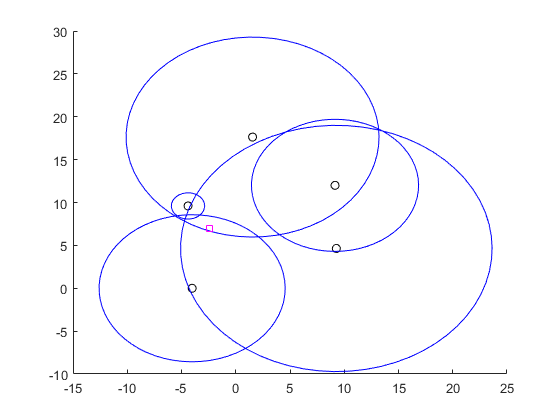
\includegraphics[scale = 0.7]{ct_1}
		\caption{Resultado gráfico do Caso de Teste 1}
	\end{figure}

	\subparagraph{Discussão}
	Neste caso, o teste convergiu para o valor esperado com dada precisão. É possível
	visualizar no resultado gráfico a estimativa da posição da fonte emissora na interseção
	da maior quantidade de receptores, o que infere uma boa qualidade na estimativa.

	\paragraph{Caso de Teste 2}: Posição Real do Emissor: ($3.00$, $3.00$).
	\subparagraph{Arquivo de Entrada das Potências}
	\begin{Verbatim}[fontsize=\footnotesize]
		p1 p2 p3 p4 p5
		-46.9 -46.4 -41.2 -45.8 -48.7
	\end{Verbatim}

	\subparagraph{Resultado Obtido}
	\begin{Verbatim}[fontsize=\footnotesize]
		0.7646725892734015773152996447686
  	8.438517018906009038428898093488
	\end{Verbatim}

	\subparagraph{Resultado Gráfico}
	\begin{figure}[h]
		\centering
		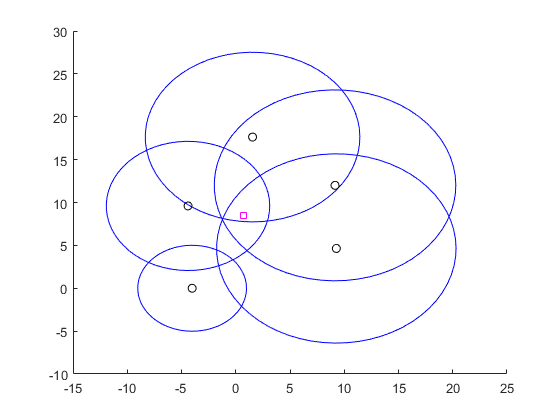
\includegraphics[scale = 0.7]{ct_2}
		\caption{Resultado gráfico do Caso de Teste 2}
	\end{figure}

	\subparagraph{Discussão}
	Neste caso, o teste não convergiu para o valor esperado com dada precisão. Pela
	análise dos valores estima-se que tenha ocorrido uma discrepância significativa
	entre os dados coletados pelos receptores, visto que a posição esperada não foi
	atingida em nenhuma das coordenadas analisadas. Isso pode significar uma falha
	decorrente de variações do ambiente ou limitações gerais, conforma abordado nas
	Seções \ref{sec:lim} e \ref{sec:discussao}.

	\section{Conclusão}
	\label{sec:conclusao}
	%TODO: Expor a análise a respeito do problema e como é solucionado pelo que foi proposto.


	%TODO: Corrigir as referências
	\bibliographystyle{sbc}
	\bibliography{references}
\end{document}
